\section{Experiments}
\label{sec:exp}
\subsection{Setup}
\label{sec:setup}
\textbf{Methods.} All LLM-based methods use the same model (Claude Opus~5.5 through the Claude Code CLI with default
sampling), the same task text, interface description, PDK sheet and topology knowledge cards, and the same budgets
(Section~\ref{sec:bench}). \emph{AnalogCoder-style}~\cite{lai2025analogcoder}: the LLM writes a design plan and a
sized netlist and revises it from simulator feedback (spec table, errors, zero-current devices, failing PVT
conditions). \emph{Gen+TPE} (AnalogCoder-Pro-style~\cite{lai2026analogcoderpro}): the LLM proposes a parameterised
topology with bounds, TPE~\cite{bergstra2011tpe,akiba2019optuna} sizes it over raw $W/L/R/C$, and up to three
regenerations receive the best result; for robust tasks TPE optimises the worst case over TT, SS/125\,$^\circ$C and
FF/$-40\,^\circ$C. \emph{Gen+CMA-ES} replaces TPE by CMA-ES to separate optimiser from parameterisation.
\emph{SPECTRA-min} is the decisive ablation: one planning call (plus at most two calls to fix program errors), then
intent-space CMA-ES with the whole budget and SPECTRA's PVT loop, but no diagnosis and no LLM repair.
\emph{Oracle} optimises the benchmark's own reference template with CMA-ES under the same budget---privileged
information that bounds what sizing alone achieves on certified tasks.

\textbf{Protocol.} Each method runs 3 seeds per task; success is decided by independent re-verification
(Section~\ref{sec:bench}). Confidence intervals are 95\% cluster bootstraps over tasks; paired comparisons use the
Wilcoxon signed-rank test on per-task success rates with Holm correction.


\subsection{Main Results}
\label{sec:main}
\IfFileExists{tables/main.tex}{\begin{table*}[t]
\centering
\caption{Main results on SPECTRA-Bench (3 seeds; success = independent re-verification at TT, or on all 45 PVT conditions for robust tasks). Calls/Sims: medians over successful runs; \$/run: mean LLM cost.}
\label{tab:main}
\small
\begin{tabular}{@{}lccccccccc@{}}
\toprule
Method & Success (\%) [95\% CI] & T1 & T2 & T3 & Robust & Designer & Calls$^\star$ & Sims$^\star$ & \$/run \\
\midrule
\textbf{SPECTRA} & 98 [94,100] & 100 & 100 & 100 & 100 & 95 & 2.0 & 2.0 & 0.40 \\
SPECTRA-min (1 call + intent CMA-ES) & 90 [77,100] & 67 & 100 & 89 & 100 & 90 & 2.0 & 1.0 & 0.26 \\
AnalogCoder-style~\cite{lai2025analogcoder} & 92 [78,100] & 100 & 100 & 67 & 100 & 100 & 1.0 & 1.0 & 0.33 \\
Gen+TPE (AnalogCoder-Pro-style)~\cite{lai2026analogcoderpro} & 90 [73,100] & 100 & 100 & 100 & 33 & 86 & 1.0 & 7.0 & 0.14 \\
\bottomrule
\end{tabular}
\end{table*}
}{}
Table~\ref{tab:main} summarises \SpectraNruns{} runs per method. SPECTRA reaches \SpectraSucc{} overall
success, versus \DirectSucc{} for the AnalogCoder-style agent, \GenboSucc{} for Gen+TPE and \SpectraMinSucc{} for
SPECTRA-min. Consistent with our pilot, the easier tiers are nearly saturated by every method---a frontier LLM can
already design a textbook amplifier to loose specifications---and the differences open where specifications are
close to the frontier: on T3, SPECTRA solves \SpectraTThree{} of runs against \DirectTThree{} (AnalogCoder-style),
\GenboTThree{} (Gen+TPE) and \SpectraMinTThree{} (SPECTRA-min). The AnalogCoder-style agent's failures are
dominated by near misses on precisely the quantities that require numerical closure (CMRR, PSRR, power), which it
cannot tune by rewriting widths; generate-then-optimise baselines fail when the proposed parameterisation or
topology cannot reach the spec, which no amount of TPE fixes. \IfFileExists{figs/E1_tiers.pdf}{Fig.~\ref{fig:tiers}
breaks success down by tier.}{}
\IfFileExists{figs/E1_tiers.pdf}{\begin{figure}[t]\centering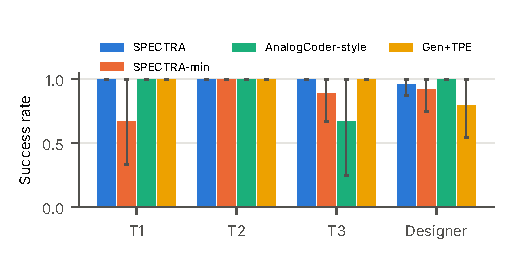
\includegraphics[width=\columnwidth]{figs/E1_tiers.pdf}
\vspace{-6mm}\caption{Success by tier (95\% cluster-bootstrap CIs over tasks).}\label{fig:tiers}\end{figure}}{}

\subsection{Ablations: What Matters?}
\label{sec:ablation}
% RESULTS-ABLATION

\subsection{PVT Closure and Mismatch}
\label{sec:pvt}
% RESULTS-PVT

\subsection{Diagnosis Accuracy under Fault Injection}
\label{sec:fault}
We inject single faults of seven classes into the reference designs of the certified tasks (undersized width,
too-short channel, wrong mirror ratio, collapsed compensation capacitor, starved bias device, miswired gate, wrong
resistor) and keep the \FaultN{} cases that violate at least one specification. Three diagnosers rank the
corrupted element: a rule-only diagnoser that scores elements by operating-region flags and element-level
sensitivities (no LLM), and the LLM given either the netlist with the specification table (the feedback used by
AnalogCoder-style agents) or the netlist with SPECTRA's diagnosis. Table~\ref{tab:fault} shows that the LLM is
far better than the rules (\FaultRawTopOne{} vs.\ \FaultRuleTopOne{} top-1) and that, for the strongest model,
SPECTRA's evidence does not raise top-1 localisation overall (\FaultDiagTopOne{}) but helps on faults whose
signature is in the operating point---mirror ratios and short channels---and raises top-3 accuracy to
\FaultDiagTopThree{}. \FaultHaikuSentence{} More evidence is therefore not automatically better: a long
structured report can distract a smaller model. We consequently treat the diagnosis as an input to the repair
\emph{decision} (refine vs.\ edit), whose end-to-end value is measured by the ablation in
Section~\ref{sec:ablation}, not as a stand-alone localiser.
\IfFileExists{tables/fault.tex}{\begin{table}[t]
\centering
\caption{Fault localisation accuracy (top-1/top-3, \%) by injected fault class: rule-only diagnoser vs.\ LLM given the netlist and spec table (raw) or the SPECTRA diagnosis.}
\label{tab:fault}
\scriptsize
\setlength{\tabcolsep}{2.5pt}
\begin{tabular}{@{}lcccc@{}}
\toprule
Fault class & $n$ & Rules & GPT-6.1-sol+raw & GPT-6.1-sol+diag. \\
\midrule
Undersized $W$ & 41 & 37/51 & 76/93 & 68/93 \\
Short $L$ & 11 & 18/73 & 73/91 & 73/82 \\
Mirror ratio & 28 & 32/61 & 86/86 & 82/89 \\
Comp.\ cap & 3 & 0/0 & 67/67 & 67/67 \\
Bias starved & 27 & 44/59 & 63/89 & 63/93 \\
Miswired gate & 44 & 36/68 & 98/100 & 95/100 \\
Resistor value & 12 & 17/75 & 75/92 & 58/83 \\
\midrule
All & 166 & 34/61 & 81/92 & 77/92 \\
\bottomrule
\end{tabular}
\end{table}
}{}

\subsection{Backbone Scaling and Cost}
\label{sec:scaling}
% RESULTS-SCALING
